\subsection{AHTR Moltres Temperature Model}
\begin{frame}
    \frametitle{AHTR Temperature Model}
    \begin{block}{AHTR Temperature Model}
        \begin{itemize}
            \item I used the open-source MSR simulation tool, Moltres, to conduct AHTR
            full assembly multiphysics simulations 
            \item AHTR Moltres simulations captures thermal feedback effects, absent
            from the purely neutronics OpenMC simulations
            \item I model the steady-state temperature of a 2D x-y AHTR cross-section
        \end{itemize}
    \end{block}
    \begin{block}{Assumptions}
        \begin{itemize}
            \item Conductive heat transfer 
            \item Heat removal by uniform salt flow in coolant regions
        \end{itemize}
    \end{block}

\end{frame}

\begin{frame}
    \frametitle{AHTR Temperature Model Setup}
    \begin{block}{Steps to produce Moltres AHTR Temperature Model}
        \begin{itemize}
          \item OpenMC neutronics model produces group constants data 
          \item Mesh generation
          \item Run Moltres model to calculate temperature distribution 
          (accepts group constants data and mesh)
        \end{itemize}
    \end{block}
    For successful AHTR Moltres simulation, I must establish suitable spatial and
    energy homogenization that preserves accuracy while maintaining an acceptable
    runtime
    \begin{block}{Energy Homogenization}
        \begin{table}[]
            \centering
            \begin{minipage}[c]{0.6\textwidth}
                \centering
                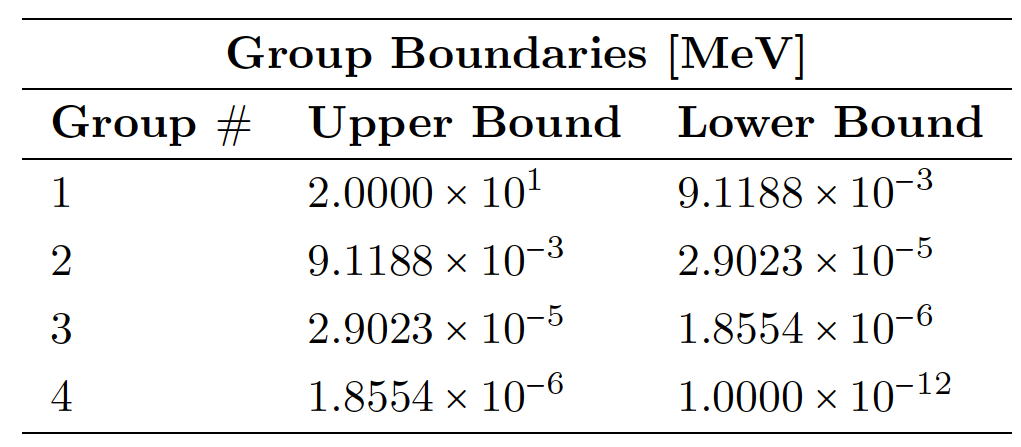
\includegraphics[width=0.8\linewidth]{figures/ahtr-energy-discr.png}
            \end{minipage}\hfill
            \begin{minipage}[c]{0.4\textwidth}
            \caption{4-group energy structures for AHTR geometry 
            derived by \cite{gentry_development_2016}.}
        \end{minipage}
        \end{table}
    \end{block}
\end{frame}

\begin{frame}
    \frametitle{AHTR Temperature Model Spatial Homogenization}
        \textbf{Fuel assembly 61 cell discretization}: inter-assembly FLiBe, 
        Y-shaped graphite structure, control rod slot FLiBe, graphite spacers, 
        each diamond shape section's inter-plank FLiBe (3), each graphite plank (18), 
        and each fuel stripe (36)
    \begin{figure}[]
            \centering
            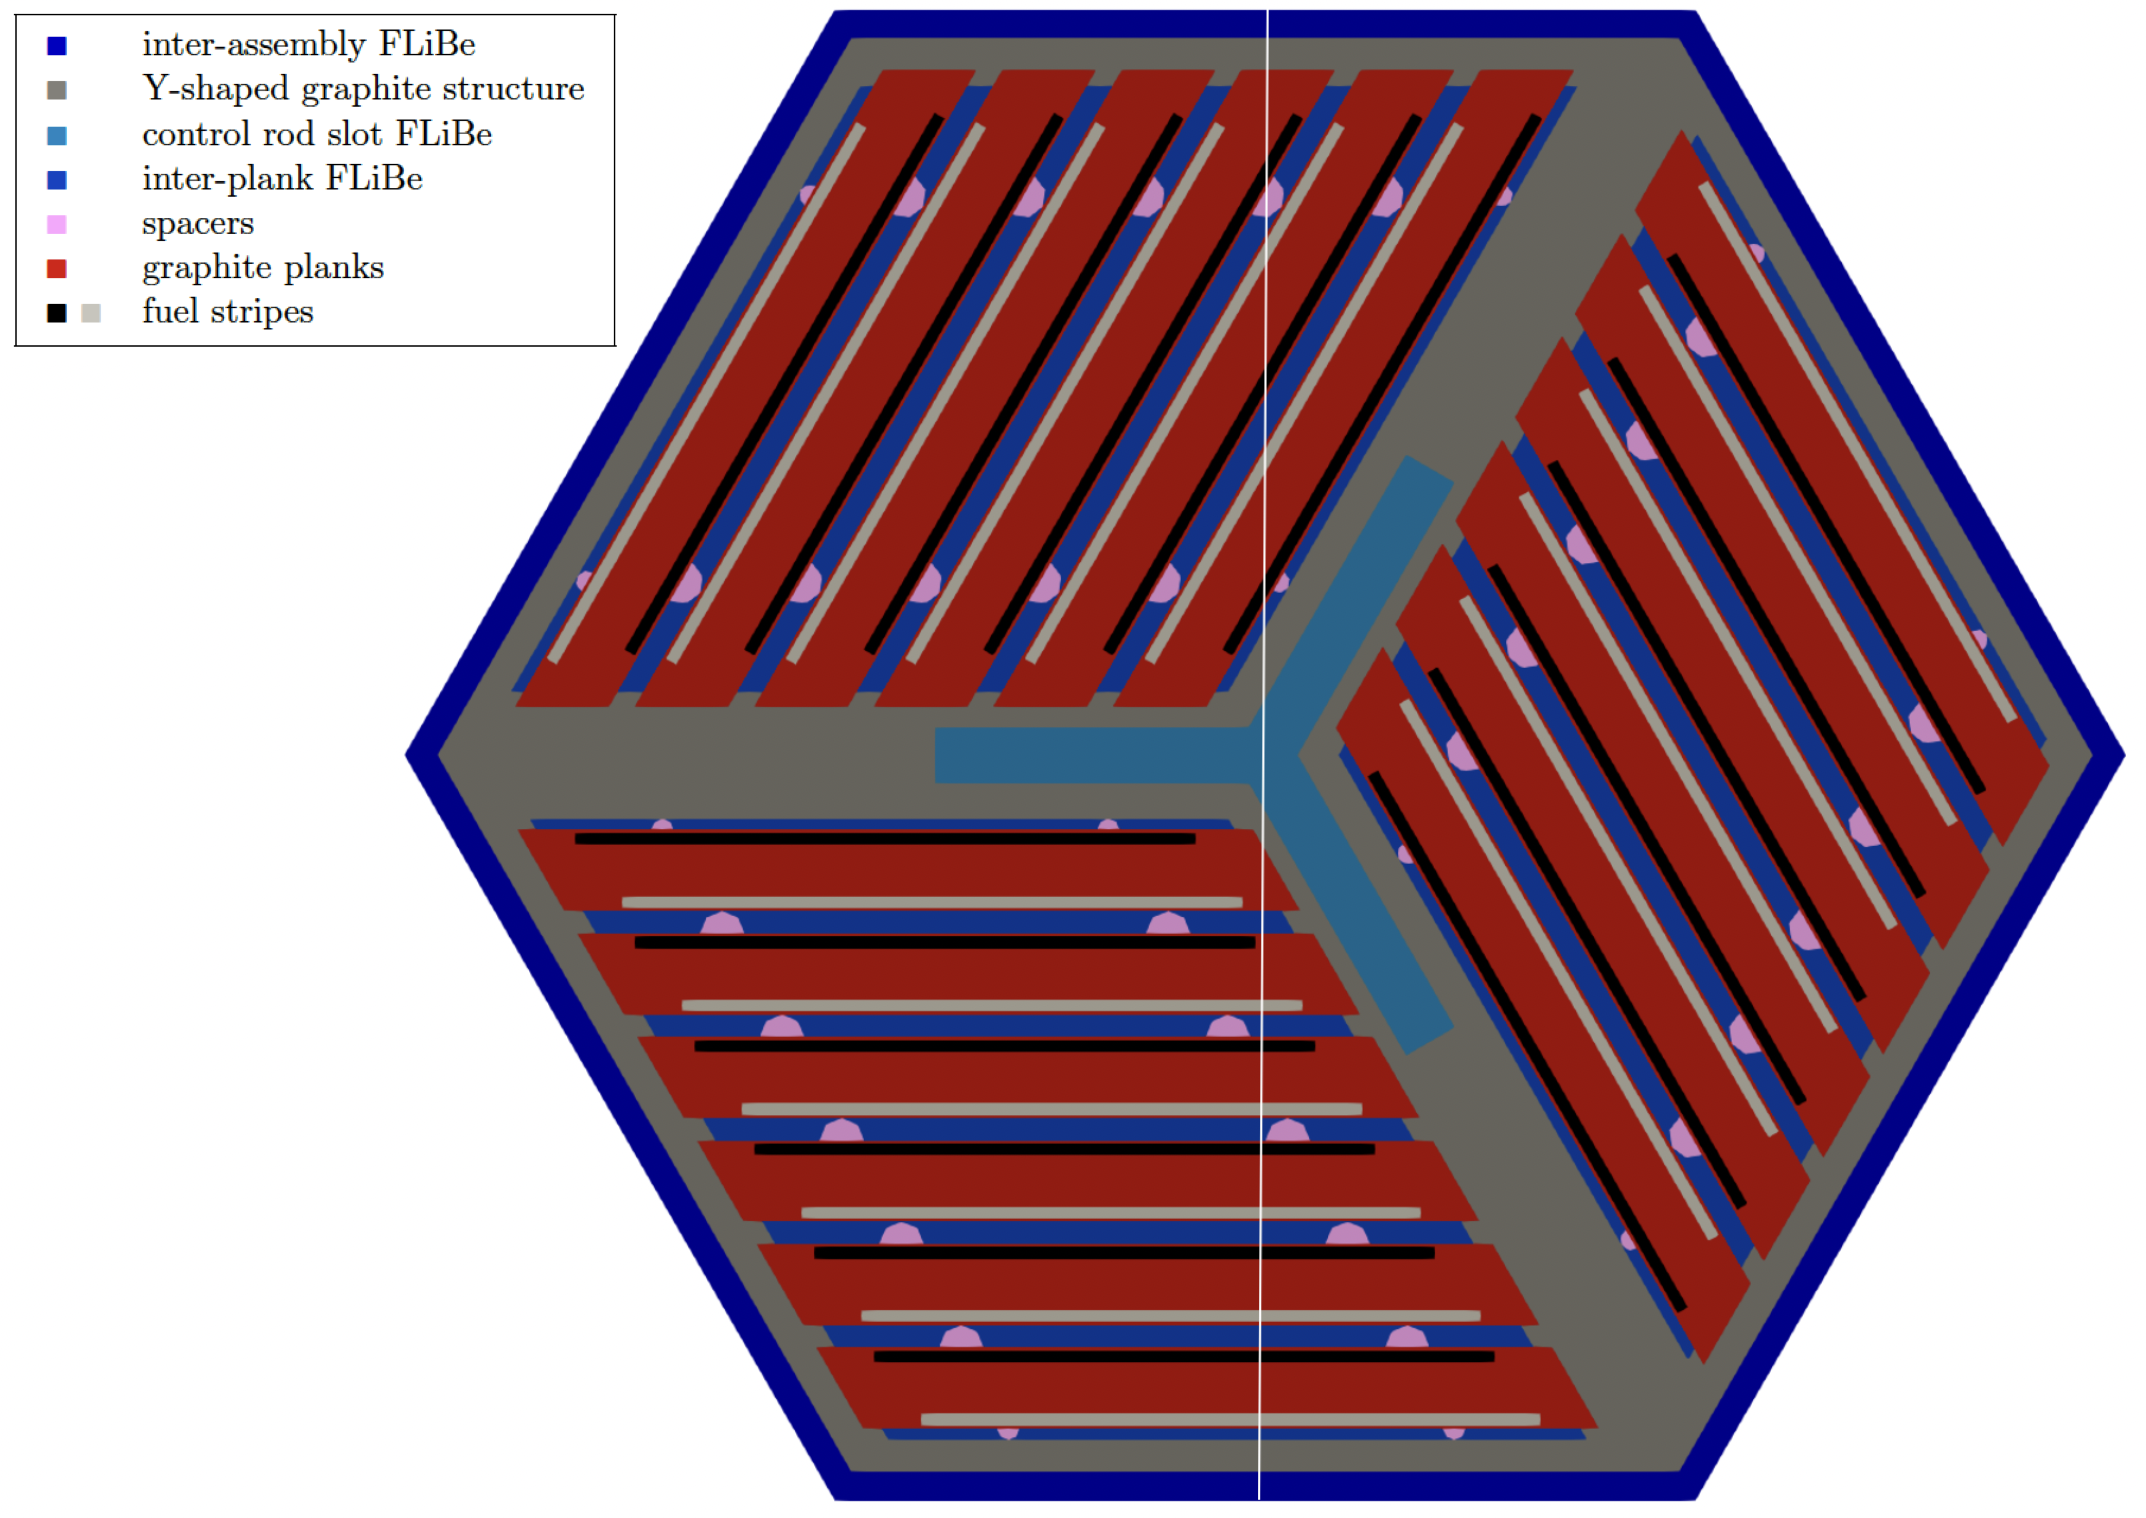
\includegraphics[width=0.65\linewidth]{figures/assembly_mg_pres.png}
        \caption{AHTR Assembly Spatial Homogenization for Group Constant Generation.}
    \end{figure}
\end{frame}

\subsection{Key Neutronics Parameters Verification}
\begin{frame}
    \frametitle{AHTR Temp Model Key Neutronics Parameter Verification}
    I \textbf{verify acceptable spatial homogenization and energy discretization} by 
    comparing key neutronics parameters (KNPs) between: 
    \begin{itemize} 
        \item OpenMC simulation with continuous energy and TRISO-level spatial fidelity
        \item Moltres simulation with 4-group energy and spatial homogenization
    \end{itemize}
    \textbf{KNPs}: $k_{eff}$, reactivity coefficients, flux distribution, and neutron spectrum. 
        \begin{table}
            \caption{ $k_{eff}$ comparison.}
            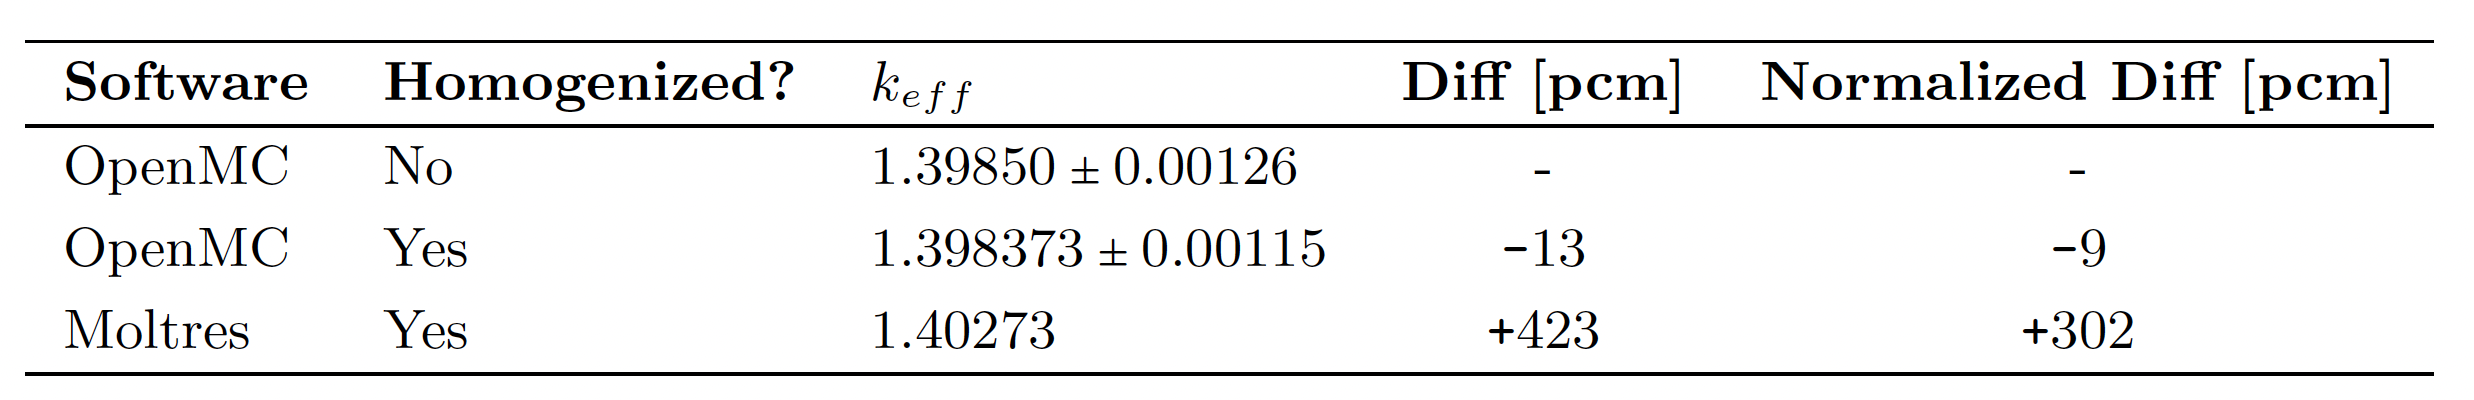
\includegraphics[width=0.85\linewidth]{figures/benchmark-keff.png}
        \end{table}
        \begin{table}
            \caption{Reactivity coefficients comparison.}
            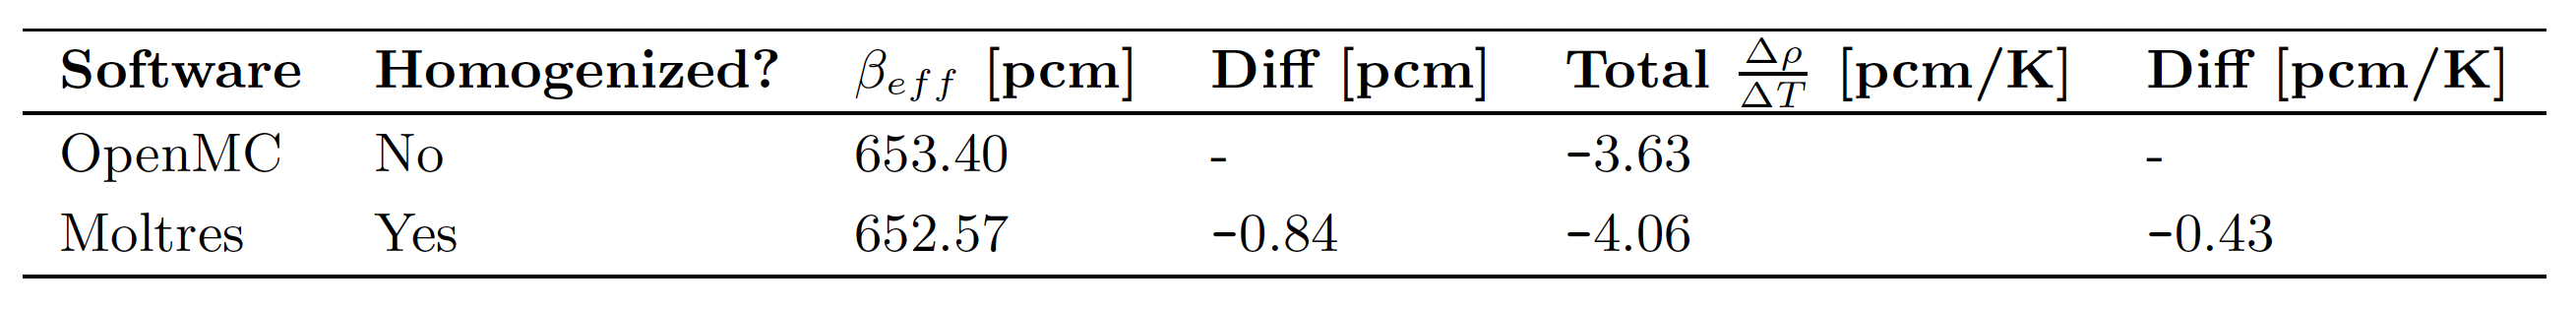
\includegraphics[width=0.85\linewidth]{figures/benchmark-coeff.png}
        \end{table}
\end{frame}

\begin{frame}
    \frametitle{AHTR Temp Model Flux Verification}
    \begin{figure}[]
        \centering
        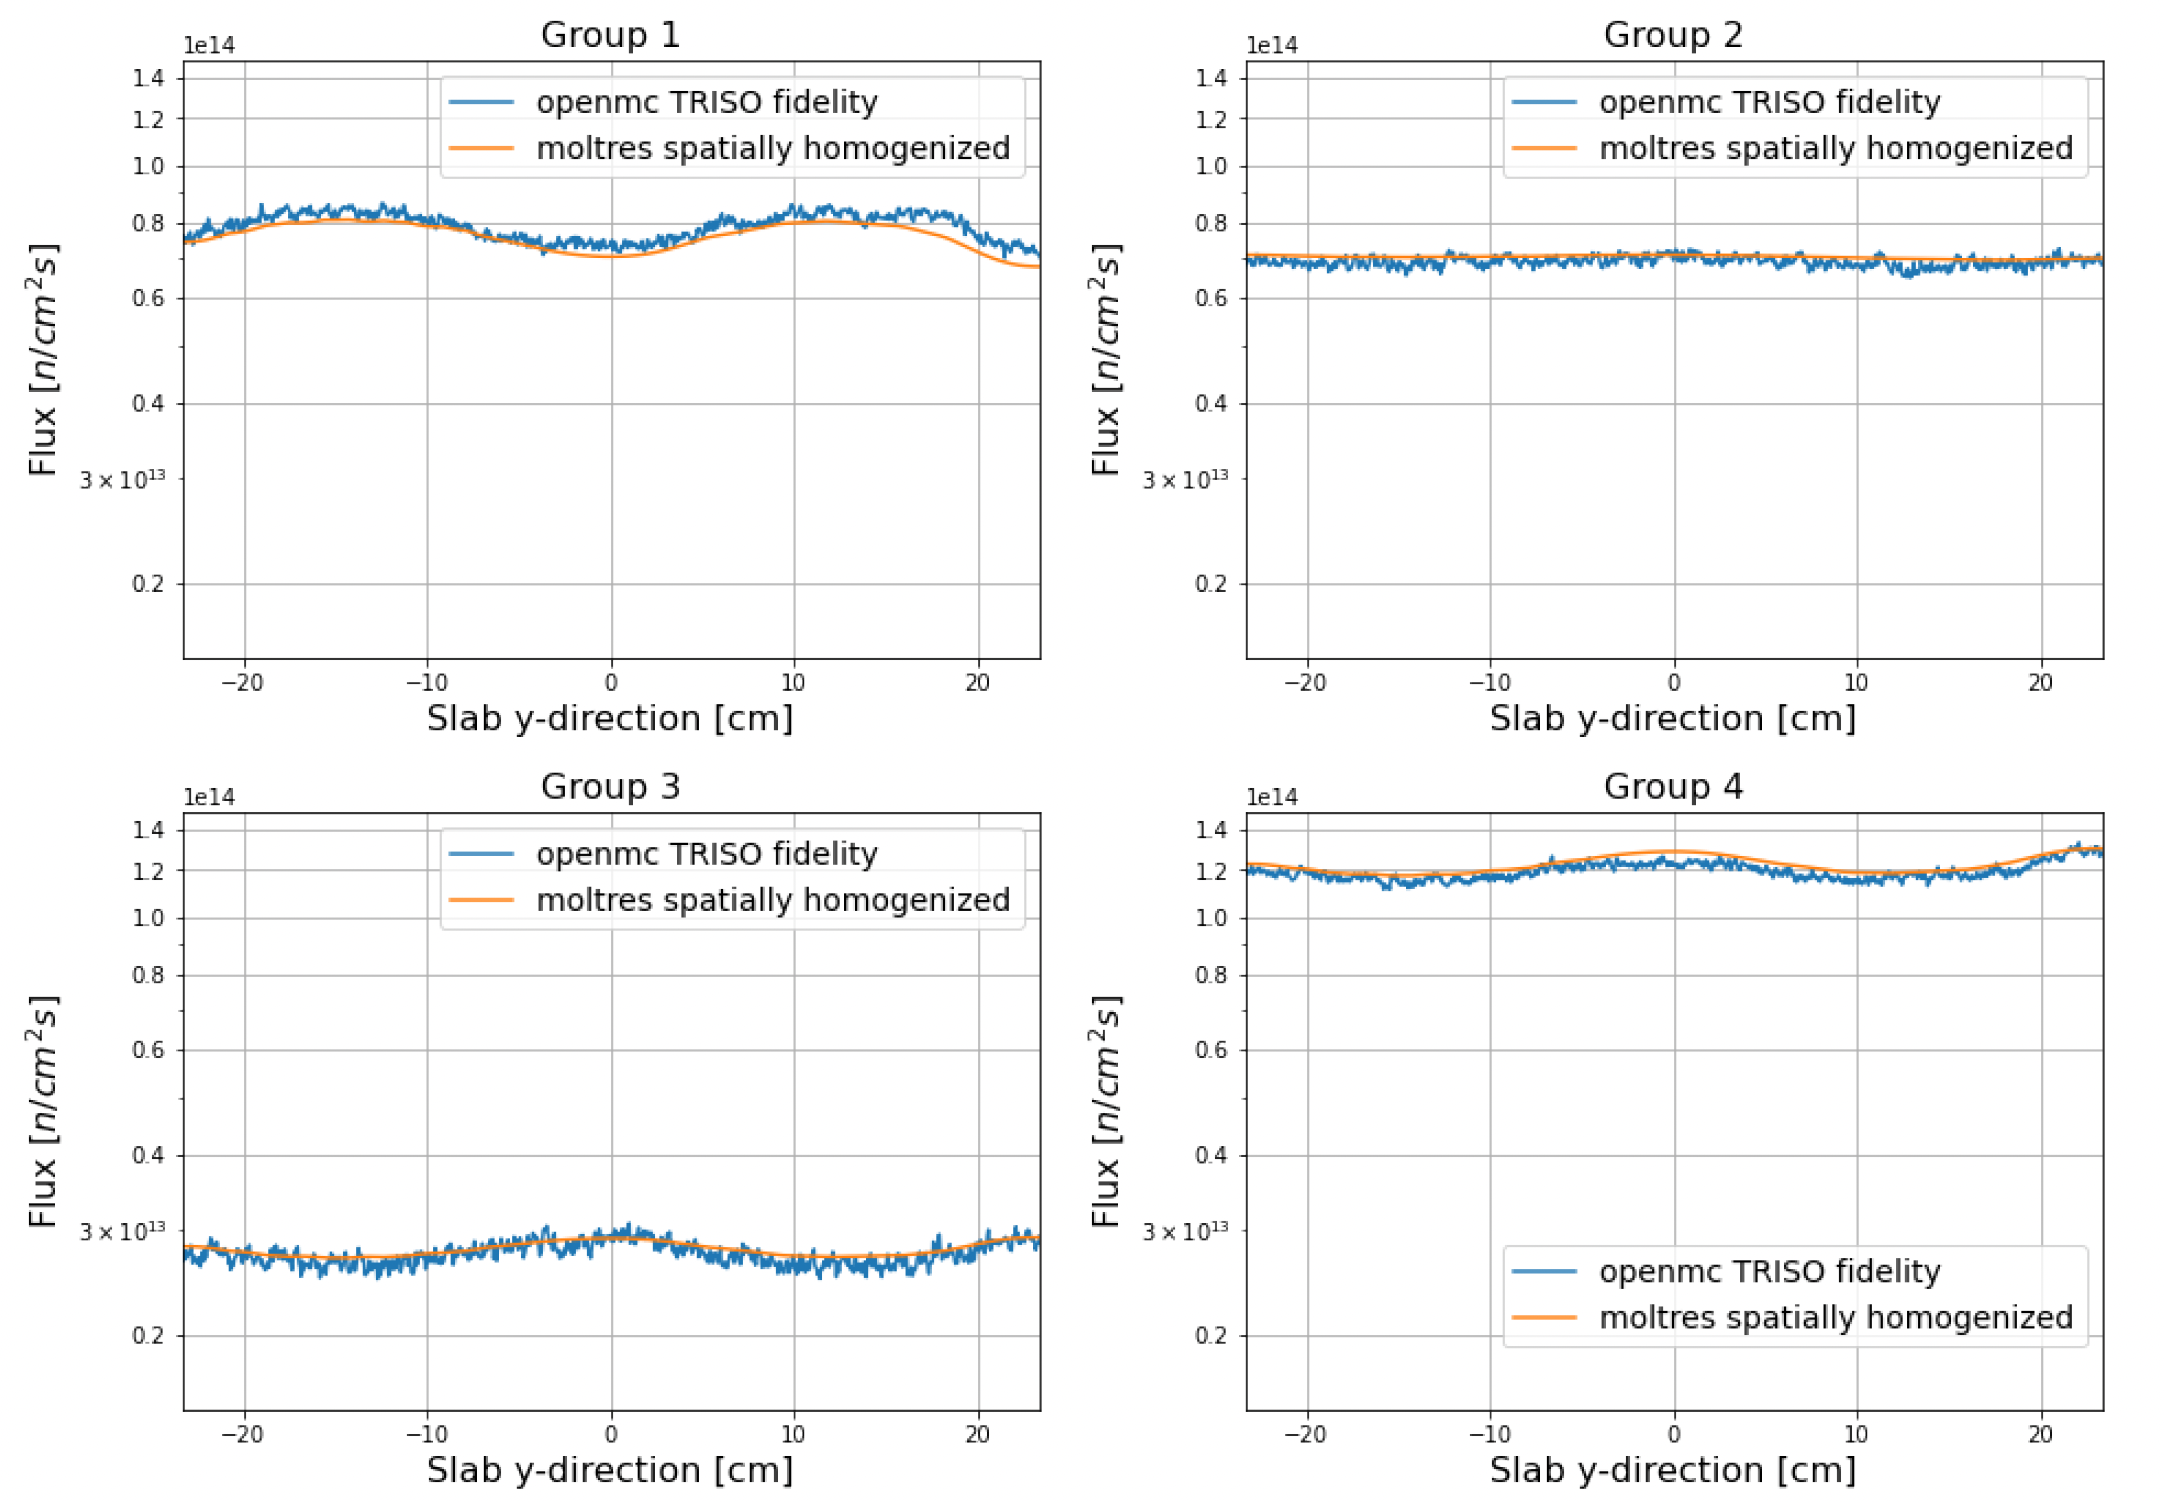
\includegraphics[width=0.8\linewidth]{figures/benchmark-flux.png} 
        \caption{4-group flux distribution comparison.}
    \end{figure}
\end{frame}

\begin{frame}
    \frametitle{AHTR Temp Model Neutron Spectrum Verification}
            \begin{figure}[]
                \centering
                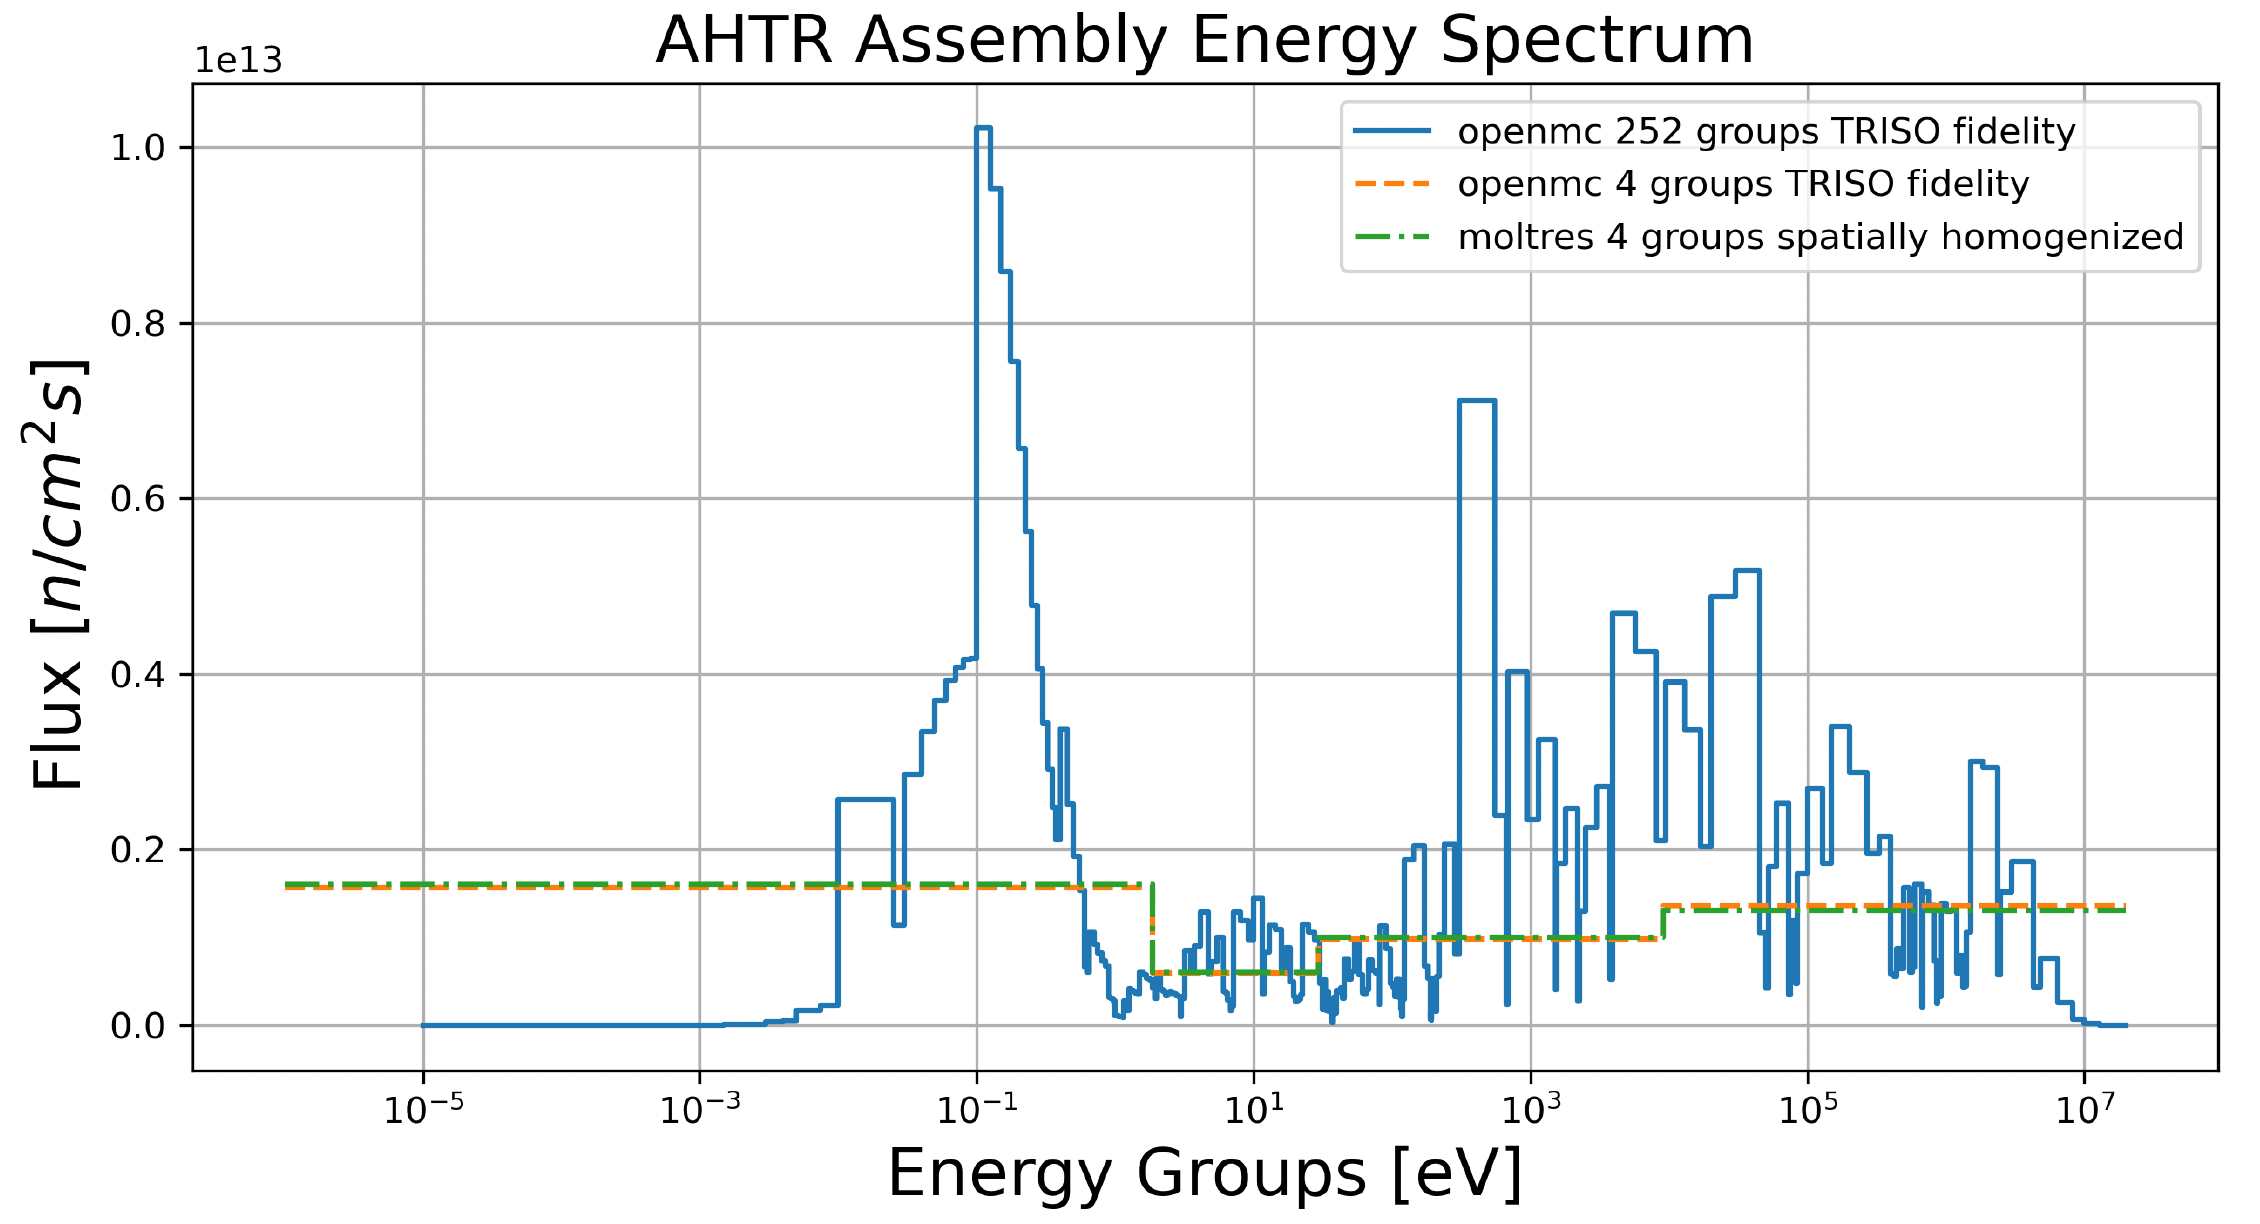
\includegraphics[width=0.75\linewidth]{figures/benchmark-spectrum.png} 
                \caption{Neutron Energy Spectrum Comparison.}
            \end{figure}
        Moltres replicated the relevant neutronics parameters with sufficient accuracy
        using OpenMC's group constant data for the AHTR full assembly model.
\end{frame}

\subsection{AHTR Temperature Model Results}
\begin{frame}
    \frametitle{AHTR Temperature Model Results}
    \begin{columns}
        \begin{column}{0.6\textwidth}
            \begin{figure}[]
                \centering
                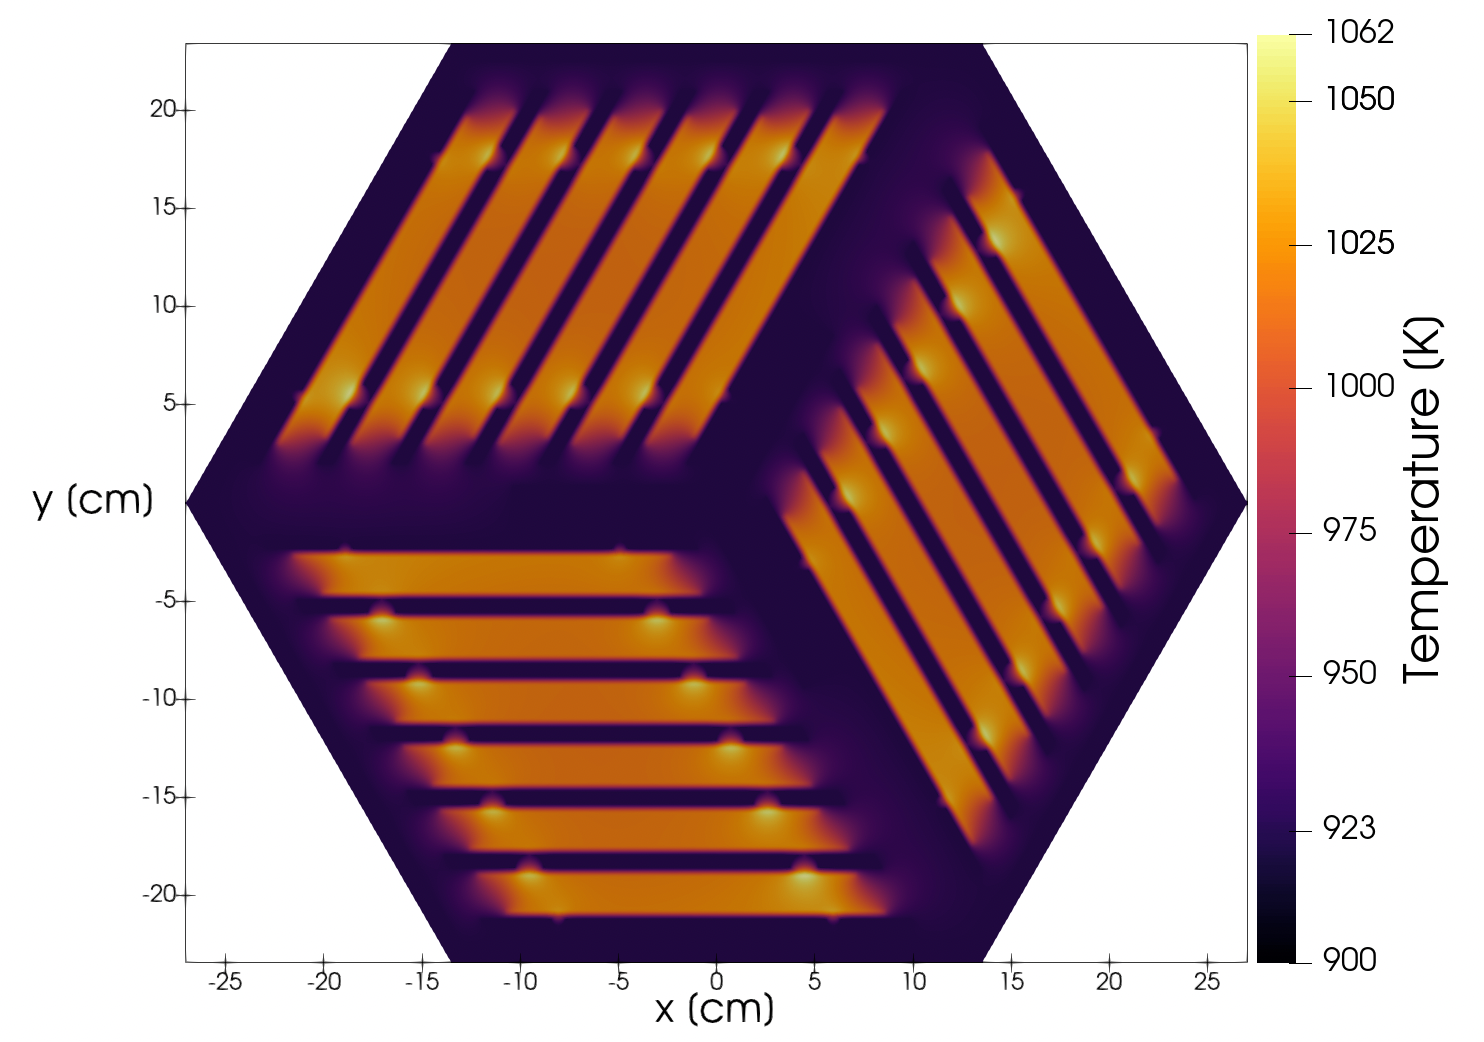
\includegraphics[width=\linewidth]{../docs/figures/benchmark-temperature-model.png} 
                \caption{2D temperature distribution in the \acrfull{AHTR}
                full assembly generated by Moltres.}
            \end{figure}
        \end{column}
        \begin{column}{0.4\textwidth} 
            \begin{block}{Results}
                \begin{itemize}
                    \item Average temperature distribution across the fuel planks are 
                    $\sim 1025K$
                    \item Average temperature of graphite structure is $\sim 935K$
                    \item Temperature peaks at 1062K in the fuel stripes near the spacers
                    \item This could be due to the extra moderation provided by the
                    graphite spacers
                \end{itemize}
            \end{block}
        \end{column}
        \end{columns}
\end{frame}

\subsection{FHR Benchmark + AHTR Model Development: Summary}
\begin{frame}
    \frametitle{FHR Benchmark + AHTR Model Development: Summary}
    \begin{block}{Major Takeaways}
        \begin{itemize}
            \item AHTR has passive safety behavior with negative temperature coeffcients
            \item Increased fuel packing does not always correspond with increased 
            $k_{eff}$ due to self-shielding effects 
            \item These results hint at the possibility of minimizing fuel required by 
            optimizing for heterogenous fuel distributions within the core
            \item AHTR temperature peaks in the fuel stripes near the spacers 
        \end{itemize}
    \end{block}
    \begin{block}{I Successfully Completed AHTR Model Development Research Objectives}
        \begin{itemize}
            \item I furthered our understanding of the AHTR design's complexities 
            through neutronics and multiphysics modeling
            \item I participated in the OECD-NEA's FHR Benchmark Phases I-A and I-B
        \end{itemize}
    \end{block}
\end{frame}
